% $Header: /home/vedranm/bitbucket/beamer/solutions/conference-talks/conference-ornate-20min.en.tex,v 90e850259b8b 2007/01/28 20:48:30 tantau $

\documentclass{beamer}

% This file is a solution template for:

% - Talk at a conference/colloquium.
% - Talk length is about 20min.
% - Style is ornate.



% Copyright 2004 by Till Tantau <tantau@users.sourceforge.net>.
%
% In principle, this file can be redistributed and/or modified under
% the terms of the GNU Public License, version 2.
%
% However, this file is supposed to be a template to be modified
% for your own needs. For this reason, if you use this file as a
% template and not specifically distribute it as part of a another
% package/program, I grant the extra permission to freely copy and
% modify this file as you see fit and even to delete this copyright
% notice. 


\mode<presentation>
{
  \usetheme{Warsaw}
  % or ...

  \setbeamercovered{transparent}
  % or whatever (possibly just delete it)
}


\usepackage[english]{babel}
% or whatever

\usepackage[latin1]{inputenc}
% or whatever

\usepackage{times}
\usepackage[T1]{fontenc}
% Or whatever. Note that the encoding and the font should match. If T1
% does not look nice, try deleting the line with the fontenc.
\usepackage{graphicx}

\title{Semi-automated point cloud cleaning}

\author{Rickert Mulder}
% - Give the names in the same order as the appear in the paper.
% - Use the \inst{?} command only if the authors have different
%   affiliation.

\institute[U of X]
{
  Department of Computer Science\\
  University of Cape Town
}

\date[CFP 2003] % (optional, should be abbreviation of conference name)
{Masters Proposal}
% - Either use conference name or its abbreviation.
% - Not really informative to the audience, more for people (including
%   yourself) who are reading the slides online

\subject{Computer Science}
% This is only inserted into the PDF information catalog. Can be left
% out. 



% If you have a file called "university-logo-filename.xxx", where xxx
% is a graphic format that can be processed by latex or pdflatex,
% resp., then you can add a logo as follows:

% \pgfdeclareimage[height=0.5cm]{university-logo}{university-logo-filename}
% \logo{\pgfuseimage{university-logo}}



% Delete this, if you do not want the table of contents to pop up at
% the beginning of each subsection:
\AtBeginSubsection[]
{
  \begin{frame}<beamer>{Outline}
    \tableofcontents[currentsection,currentsubsection]
  \end{frame}
}


% If you wish to uncover everything in a step-wise fashion, uncomment
% the following command: 

%\beamerdefaultoverlayspecification{<+->}


\begin{document}

\begin{frame}
  \titlepage
\end{frame}

\begin{frame}{Outline}
  \tableofcontents
  % You might wish to add the option [pausesections]
\end{frame}


% Structuring a talk is a difficult task and the following structure
% may not be suitable. Here are some rules that apply for this
% solution: 

% - Exactly two or three sections (other than the summary).
% - At *most* three subsections per section.
% - Talk about 30s to 2min per frame. So there should be between about
%   15 and 30 frames, all told.

% - A conference audience is likely to know very little of what you
%   are going to talk about. So *simplify*!
% - In a 20min talk, getting the main ideas across is hard
%   enough. Leave out details, even if it means being less precise than
%   you think necessary.
% - If you omit details that are vital to the proof/implementation,
%   just say so once. Everybody will be happy with that.

\section{Motivation}

\subsection{Background}

\begin{frame}{The Zamani Project}
  % - A title should summarize the slide in an understandable fashion
  %   for anyone how does not follow everything on the slide itself.

  
\includegraphics[width=0.70\textwidth]{pics/Zamani_logo}

  \begin{itemize}
  \item
    Cultural heritage preservation.
  \item
    Capture the spatial domain of heritage sites.
  \end{itemize}
\end{frame}

\begin{frame}{Capturing the Spatial Domain}
  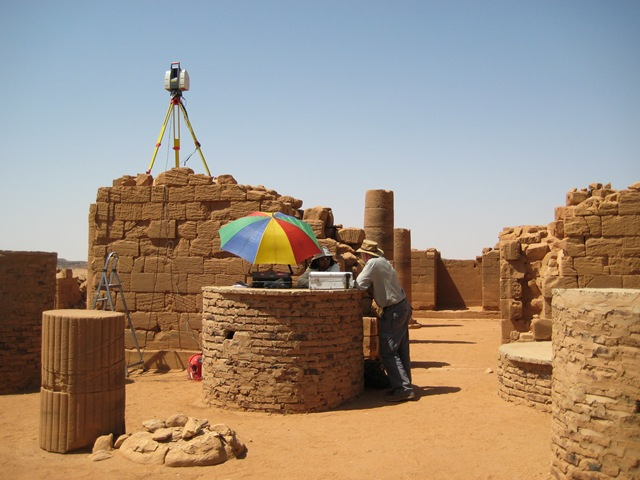
\includegraphics[width=0.60\textwidth]{pics/scanning.jpg}
    \begin{itemize}
  \item
    Laser range scanning.
  \item
    Site photography.
  \end{itemize}
\end{frame}

\begin{frame}{Processing Pipeline}
  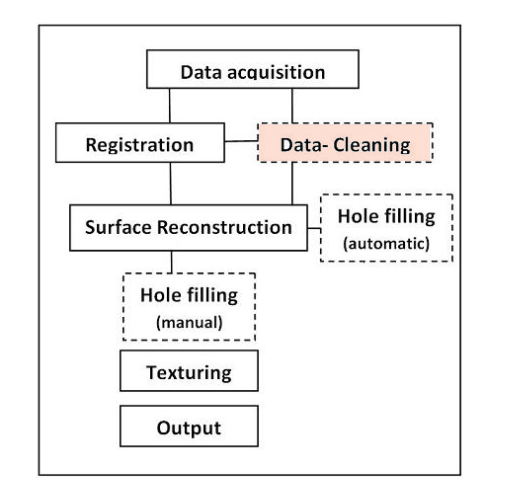
\includegraphics[width=0.50\textwidth]{pics/pipeline.png}
  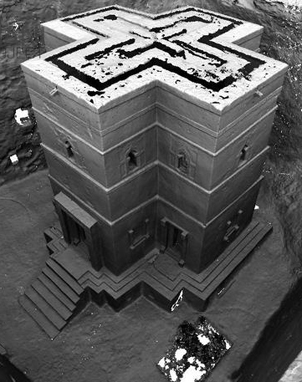
\includegraphics[width=0.38\textwidth]{pics/zamani2.jpg}
\end{frame}

\begin{frame}{Cleaning}
  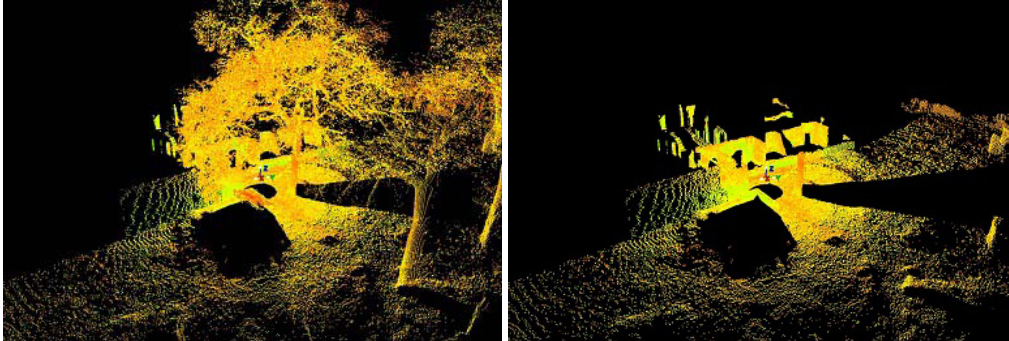
\includegraphics[width=1\textwidth]{pics/cleaning.png}
  \begin{itemize}
  \item
  Cleaning is the removal of unwanted objects.
  \item
  Involves the classification and segmentation of `noise'.
  \item
  It can happen before or after registration.
  % duplication of work
  % more memory requirements
  % size of data input should be noted
  \end{itemize}
\end{frame}

\begin{frame}{Problem}
  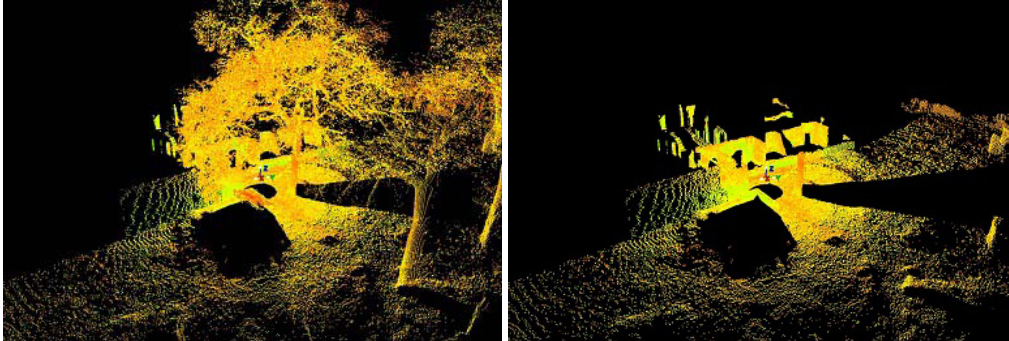
\includegraphics[width=1\textwidth]{pics/cleaning.png}
  \begin{itemize}
  \item
  Cleaning is a manual task.
  \item
  500 - 1000 scans per expedition.
  \item
  30 min to 2 hours per scan.
  % duplication of work
  % more memory requirements
  % size of data input should be noted
  % not only Zamani but also CyArk
  \end{itemize}
\end{frame}

\subsection{Previous Work}

\begin{frame}{Existing software}
% Existing software is often sluggish also
% response times plays a big role

\includegraphics[height=0.10\textheight]{pics/cyclone.jpg}

\includegraphics[height=0.10\textheight]{pics/pointools.jpg}

\includegraphics[height=0.10\textheight]{pics/meshlab.png}

\includegraphics[height=0.10\textheight]{pics/vrmesh.png}

\includegraphics[height=0.10\textheight]{pics/3dreshaper.jpg}

\vskip0pt plus.5fill

Existing tools vary in terms of
\begin{itemize}
\item automation
\item accuracy
\end{itemize}

%\begin{itemize}
%\item Leica Cyclone (used by Zamani)
%\item Pointools Edit (used by CyArk)
%\item Meshlab
%\item VR Mesh Studio
%\item Terrascan
%\item 3D Reshaper
%\item Carlson PointCloud
%\end{itemize}

\end{frame}


\begin{frame}{Simple tools}

\begin{columns}[T]
\begin{column}{0.5\textwidth}
Manual\\
High accuracy\\
\textbf{Examples:}
\begin{itemize}
\item Point picking.
\item Rectangle select.
\item Lasso tool.
\item 3D selection brushes.
\end{itemize}

\end{column}
\begin{column}{0.5\textwidth}
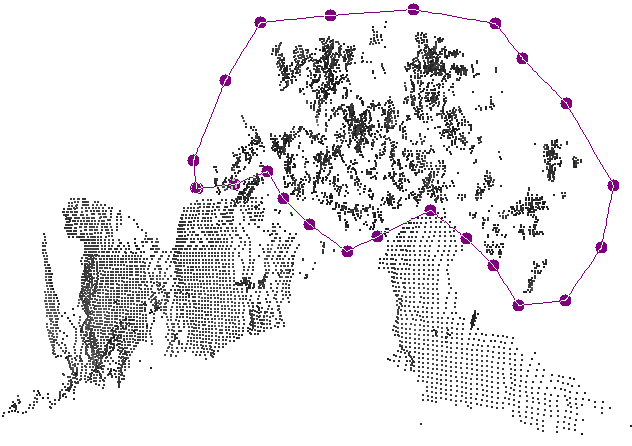
\includegraphics[width=1\textwidth]{pics/lasso.png}
\end{column}

\end{columns}

\end{frame}

\begin{frame}{Semi-automated tools}


\begin{columns}[T]
\begin{column}{0.5\textwidth}

Manual\\
Varying accuracy\\
Not suitable for all artefacts\\
\textbf{Examples:}
\begin{itemize}
\item Plane select.
\item Region growing based on:

\begin{itemize}
\item Point intensity or colour value.
\item Point normals.
\item Distance.
\end{itemize}

\item Specialised selections.
\begin{itemize}
\item Power lines.
\item Fire hydrants.
\end{itemize}
\end{itemize}

\end{column}
\begin{column}{0.5\textwidth}
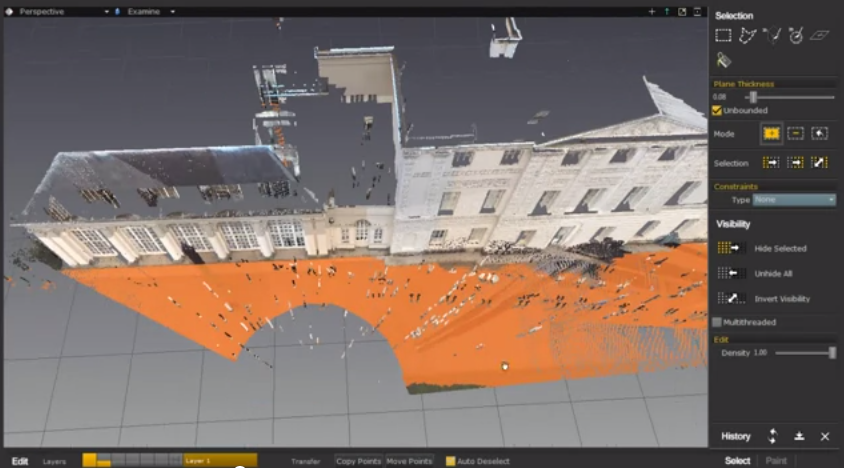
\includegraphics[width=1\textwidth]{pics/plane.png}
\end{column}

\end{columns}

\end{frame}


\begin{frame}{Fully automated}

\begin{columns}[T]
\begin{column}{0.5\textwidth}

Automatic\\
Low accuracy\\

\textbf{Examples:}
\begin{itemize}
\item Isolated point removal.
\item Point clustering based on:
\begin{itemize}
\item Distance.
\item Colour/Intensity.
\end{itemize}
\item Classification of:
\begin{itemize}
\item Ground.
\item Roofs.
\item Vegetation.
\item XYZ planes.
\end{itemize}

\end{itemize}

\end{column}

\begin{column}{0.5\textwidth}

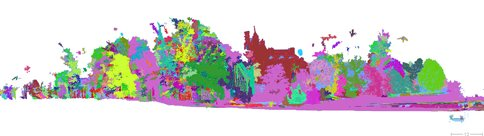
\includegraphics[width=1\textwidth]{pics/3DReshaper_auto_pt_cloud_seg.jpg}

\end{column}
\end{columns}

\end{frame}

\begin{frame}{Issues}

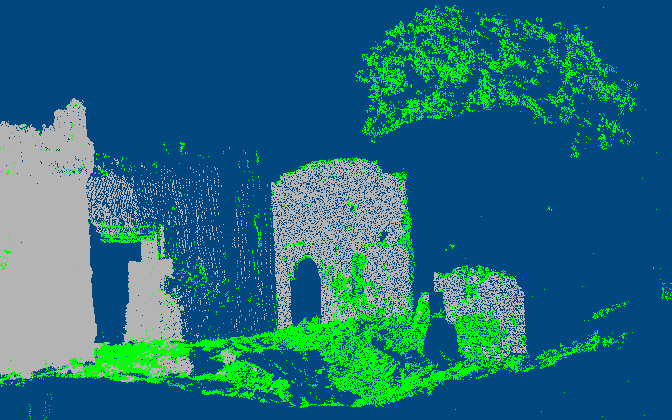
\includegraphics[width=0.50\textwidth]{pics/vrmesh-veg.png}
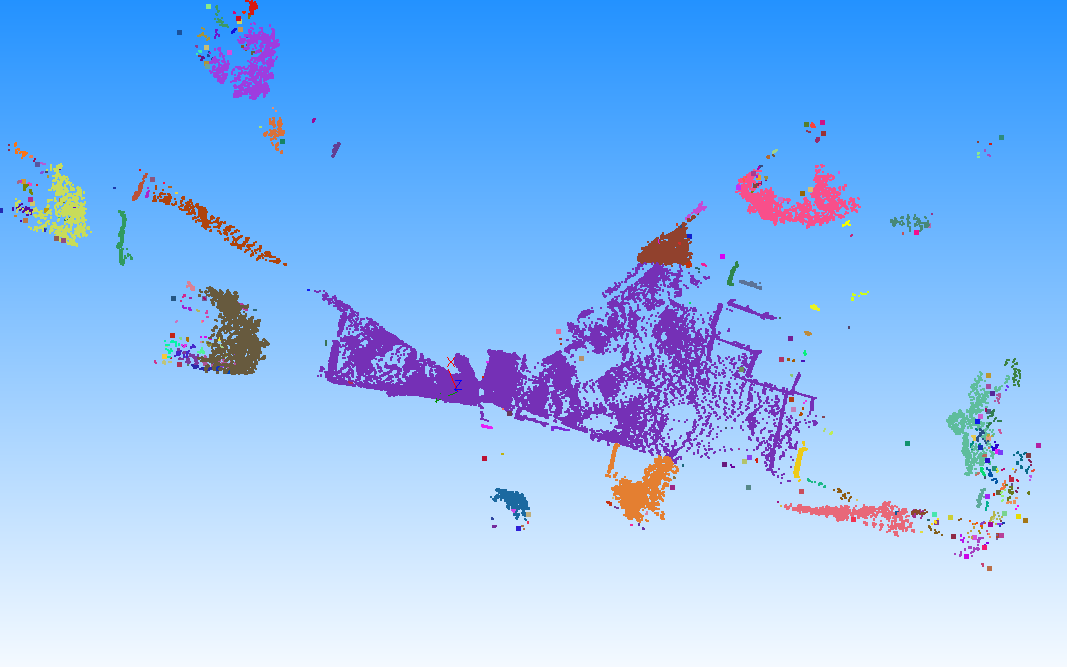
\includegraphics[width=0.50\textwidth]{pics/clustering.png}

\begin{itemize}
\item Noisy structures.
\item Non uniform point cloud density.
\end{itemize}

% Distance clustering breaks down
% Fully automated appoaches have trouble with noisy buidlings

\end{frame}

\begin{frame}{General classification}

\begin{columns}[T]
\begin{column}{0.5\textwidth}

\begin{enumerate}
\item Calculate point features.
\item Classify points:
\begin{itemize}
\item Heuristics.
\item Probabilistic models.
\end{itemize}
\end{enumerate}

\end{column}

\begin{column}{0.5\textwidth}


\includegraphics[width=1\textwidth]{pics/segmentation.png}

\end{column}

\end{columns}


\end{frame}

\begin{frame}{Point feature algorithms}

\begin{columns}[T]
\begin{column}{0.5\textwidth}

\textbf{Examples:}
\begin{itemize}
\item Point normals.
\item Fast point feature histograms.
\item Principle component analysis.
\end{itemize}

\textbf{Considerations:}
\begin{itemize}
\item Rotation invariance.
\item Scale invariance.
\item Point density invariance.
\end{itemize}

\end{column}

\begin{column}{0.5\textwidth}


\includegraphics[width=1\textwidth]{pics/features.png}

\end{column}

\end{columns}

\end{frame}

\begin{frame}{Point classification}

\begin{columns}[T]
\begin{column}{0.5\textwidth}

\textbf{Heuristic reasoning}\\
\textbf{Markov models:}
\begin{itemize}
\item Conditional Random Fields.
\item Associative Markov Networks.
\end{itemize}

% should say how they are benficial and computational cost
% expain how they work
% cleaner segmentation
% results from robotics

\end{column}

\begin{column}{0.5\textwidth}
%\vskip0pt plus.5fill
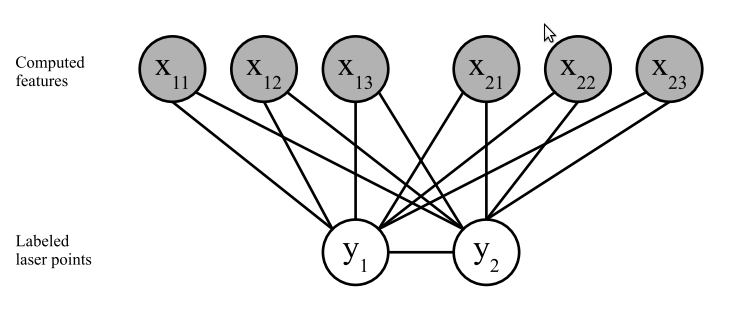
\includegraphics[width=1\textwidth]{pics/crf.png}


\end{column}

\end{columns}


\end{frame}

\section{Proposal}

\subsection{Aim}

\begin{frame}{Aim}
\begin{itemize}

\item
Produce semi-automated methods to segment point cloud artefacts in a way that is both fast and accurate.

\item
Focus on cleaning vegetation, equipment, and people.
\end{itemize}


\end{frame}

\begin{frame}{Research Questions?}

\begin{itemize}
\item To what degree can semi-automated methods speed up the point cloud cleaning process?
\item What degree of accuracy can be achieved by semi-automated segmentation methods?
\item Can probabilistic models be used to improve accuracy without significantly sacrificing performance?
\item Can probabilistic frameworks be parallelisable in order to mitigate performance penalties?  
\item Can artefact classes be dynamically learnt and used for semi-automated segmentation?
\end{itemize}

\end{frame}

\subsection{Method}

\begin{frame}{Method}

\begin{itemize}
\item Investigate:
\begin{itemize}
  \item Point features.
  \item Heuristic classification.
  \item Probabilistic classification.
  \item Machine learning.
\end{itemize}
\item Iterative Prototyping.
\item Continuous evaluation.
\end{itemize}

\end{frame}

\begin{frame}{System}

  \setlength\fboxsep{5pt}
  \setlength\fboxrule{0.0pt}

  \fbox{
\includegraphics[height=0.15\textheight]{pics/qt-logo.png}}
  \fbox{
\includegraphics[height=0.15\textheight]{pics/opencl.png}}
  \fbox{
\includegraphics[height=0.15\textheight]{pics/opengl.png}}
  \fbox{
\includegraphics[height=0.15\textheight]{pics/pcl_vert_large_pos.png}}

\begin{itemize}
\item Synthesis of semi-automated segmentation methods.
\item Facilitate fast and accurate cleaning.
\item Focus of responsiveness.
\begin{itemize}
\item Avoid transfers.
\item Push load to GPU.
\end{itemize}
\item Input:
\begin{itemize}
\item Individual scans.
\item Leica PTX format.
\item Around 16 million points. % 64 MB in memory 250 on file
\item XYZI values.
\end{itemize}

\end{itemize}

\end{frame}

\begin{frame}{Evaluation}
	\begin{itemize}
	\item Expert opinion
	\item User study to measure time and accuracy
	\begin{itemize}
	\item Timed scan cleaning task.
	\item Accuracy measured relative to a pre cleaned scan.
	\begin{itemize}
	\item Diff with precleaned cloud
	\end{itemize}
	% Point cloud diff
	\end{itemize}
	\end{itemize}

\centering
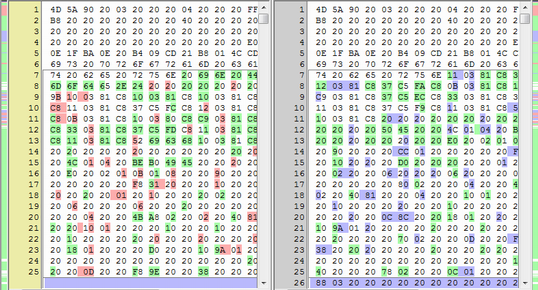
\includegraphics[width=0.5\textwidth]{pics/diff.png}

\end{frame}

\subsection{Ideas}


\begin{frame}{Feature space distance}

\begin{columns}[T]

\begin{column}{0.5\textwidth}

\begin{itemize}
\item FPFH calculates 33 bins
\item Use euclidean distance between two points in feature space for clustering in the point's neighbourhood.
\end{itemize}  

\end{column}

\begin{column}{0.5\textwidth}

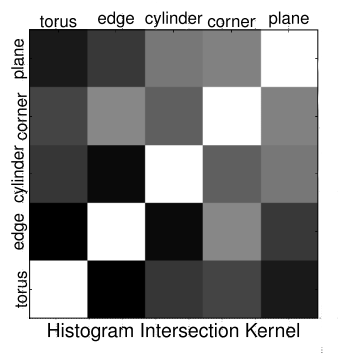
\includegraphics[width=1\textwidth]{pics/fpfh.png}

\end{column}

\end{columns}

\end{frame}


\begin{frame}{Registration based cleaning}

\begin{columns}[T]

\begin{column}{0.5\textwidth}

  Scans overlap so duplicate cleaning is required.
  \begin{enumerate}
  \item Clean scan A
  \item Register scan A to scan B
  \item Apply cleaning from scan A to scan B
  \item Clean clean scan A
  \end{enumerate}

\end{column}

\begin{column}{0.5\textwidth}

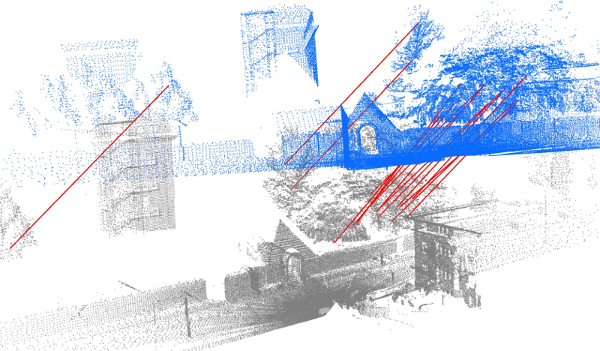
\includegraphics[width=1\textwidth]{pics/registration_outdoor.png}

\end{column}

\end{columns}

\end{frame}

\begin{frame}{Factor out distance}

\begin{columns}[T]

\begin{column}{0.5\textwidth}

A point's distance from the scanner determines:
\begin{itemize}
\item Cloud density.
\item Intensity of light returned to the scanner.
\end{itemize}

\end{column}

\begin{column}{0.5\textwidth}

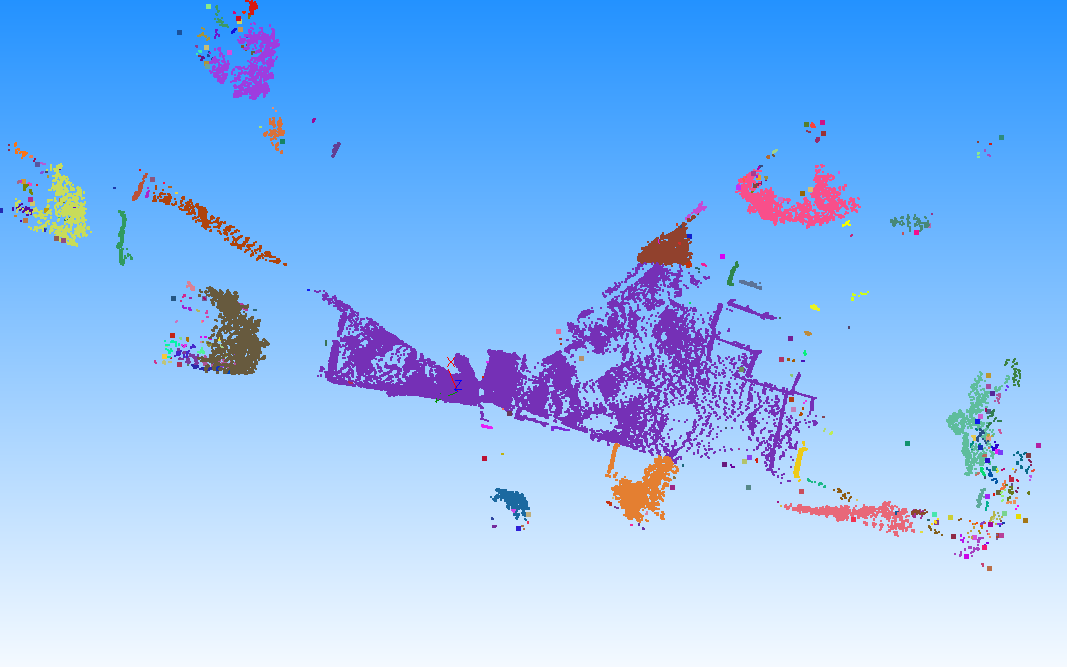
\includegraphics[width=1\textwidth]{pics/clustering.png}
% Many classification schemes does not take distance into account 

\end{column}

\end{columns}



  
\end{frame}

\section*{Summary}

\begin{frame}{Summary}

  % Keep the summary *very short*.
  \begin{itemize}
  \item
    Cleaning point clouds is time consuming.
  \item
    Speed up with semi-automated methods.
  \item
    Maintain accuracy.
  \end{itemize}
  
  % The following outlook is optional.
  %\vskip0pt plus.5fill
\end{frame}



% All of the following is optional and typically not needed. 
\appendix
\section<presentation>*{\appendixname}
\subsection<presentation>*{For Further Reading}

%\begin{frame}[allowframebreaks]
%  \frametitle<presentation>{For Further Reading}
%    
%  \begin{thebibliography}{10}
%    
%  \beamertemplatebookbibitems
%  % Start with overview books.
%
%  \bibitem{Author1990}
%    A.~Author.
%    \newblock {\em Handbook of Everything}.
%    \newblock Some Press, 1990.
% 
%    
%  \beamertemplatearticlebibitems
%  % Followed by interesting articles. Keep the list short. 
%
%  \bibitem{Someone2000}
%    S.~Someone.
%    \newblock On this and that.
%    \newblock {\em Journal of This and That}, 2(1):50--100,
%    2000.
%  \end{thebibliography}
%\end{frame}

\end{document}


